\section{An Analytic Model}\label{sec:dspmv-analytic}

This section discusses an analytic model for the SpMV algorithm run here that is modeled after the algorithm in \cite{techbib:6933066}. It assumes we compute the product $y=Ax$ where the $N~x~N$ matrix $A$ has a total of $nnz$ non-zero elements,  and where the system doing the computation is a $P=p^2$ array of MPI processes interconnected in a 2D array.

\begin{figure*}\begin{centering}
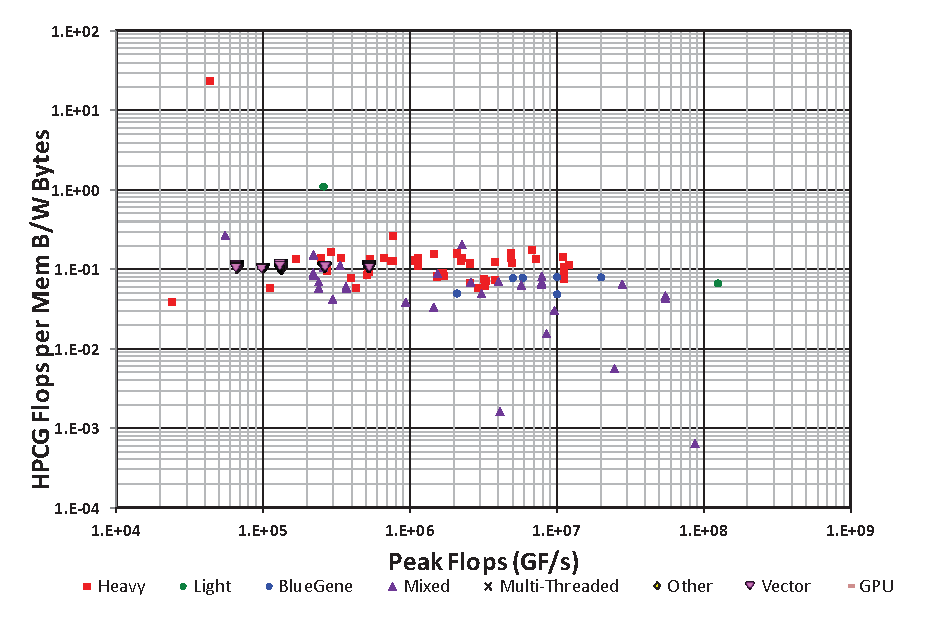
\includegraphics[scale=0.80]{figures/spmv-historical-hpcg-bw.eps}
\caption{HPCG Flops per Byte of Memory Bandwidth vs. Peak flops.}
\label{fig:spmv-historical-hpcg-bw}
\end{centering}\end{figure*}


In terms of what to expect, the performance of the HPCG benchmark \cite{techbib:hpcg-snl-dongarra} is heavily dependent on SpMV-like calculations, and work on highly accurate modeling of its performance \cite{techbib:marjanovic2014performance} led to the conclusion that HPCG's performance in terms of flops/sec was independent of the peak flop potential of the system running it, and primarily dependent on the available memory bandwidth. Fig. \ref{fig:spmv-historical-hpcg-bw} demonstrates the correctness of this conclusion by diagramming real data taken from recent HPCG reports\footnote{http://www.hpcg-benchmark.org/}. The x-axis is the peak flops of the reported system; the y-axis is the ratio of the sustained HPCG flops to the aggregate peak bandwidth of the system's memory (derived by determining the processing chips used and looking up their memory channel characteristics). The color and shape refer to different types of chips and systems, with the red squares representing system built from server-class chips, the blue representing Blue Gene, and the purple representing heterogeneous systems using GPUs. As can be seen, this ratio is independent of the peak system flops capability. In fact there is a nearly flat bounding line of a little less than 0.2 flops per byte of memory bandwidth for heavyweight server class processor chips, and somewhat less than 0.1 for GPUs and other architectures.

The model built here thus focuses on the relationship between memory bandwidth and performance in SpMV.

\subsection{Algorithm Overview}

The algorithm assumes that $A$ has been divided into $p^2$ sub-matrices of equal size $(N/p)x(N/p)$, and on average has $nnz/N$ non-zeros per row. The $N$-element column vector $x$ is assumed striped across the columns, again in equal-sized $N/p$ pieces so that all $p$ processes in a column have copies of the same segment of $x$. The column vector y is assumed stored in the first column of processes, again in stripes of $N/p$ elements per process. Each process then has all, and only, the non-zeros for the rows of A covered by the row the process is in, and all, and only, the non-zeros for the columns of A covered by the column the process is in. This is on average $nnz/Np$ non-zeros per row in each process. They are stored in a CSR (compressed sparse row) format.

In execution, each process concurrently performs its portion of the matrix-vector product, namely a $(N/p)x(N/p)$ by $N/p$ product. The resulting $N/p$ element column is sent to the process on column 0 of the process's row, and atomically added into the y vector segment stored there. Each of the processes has on average $nnz/p^2$ non-zeros in its sub-matrix, $nnz/(Np)$ of them in each of its $N/p$ row segments. Each of these non-zeros requires 2 flops (a multiply and an add), for a total of $2nnz/P$ flops performed per process. The atomic adds into the final y vector are not counted.

After the reduction, a barrier across all column 0 processes signals completion.

\subsection{Single Process}\label{sec:spmv-analytic:single}

We first look at the computation within a single MPI process using as many threads as reasonable to perform the multiply. As discussed in \cite{techbib:marjanovic2014performance} for the SpMV kernel, the processing of each row in the local matrix partition requires three memory references for each non-zero: one each for the next non-zero from $A$ and the column index for that non-zero, and an access into the $x$ vector to get the matching terms for the product. \cite{techbib:marjanovic2014performance} modeled a 4-byte index, and determined that on average about 20 bytes needed to be accessed from memory to start/finish each row, regardless of the number of non-zeros. This gave a total of $20+20nnz/Np$ bytes needed to be accessed for each row of $N/p$ elements in length. Assuming enough threads (each handling different rows) to keep the local memory busy, dividing this into 2 flops, and multiplying by the sustainable bandwidth from memory gives an initial flops/s estimate. For the HPCG modeled by \cite{techbib:marjanovic2014performance}, this seemed very accurate.

\cite{techbib:marjanovic2014performance} assumed that all these bytes needed to be physically fetched from memory, i.e. no benefits from cache reuse. This is certainly true of the non-zero and index read from memory - each such term is read exactly once during the multiply and then never reused. The access of the $x$ element needs more discussion. Given modern caches where 20MB or more may be available on-chip, depending on the number of rows of $A$, it may be possible to eventually capture all of $x$ (for example an $x$ segment of a million elements requires only 8MB of cache). Thus, if there are enough non-zeros in the partition of $A$, then the later ones are liable to find their $x$ values cached, and not require memory bandwidth.

Assuming a cache line of $B$ bytes (holding $B/8$ double floats from $x$) then a total of $(N/p)/(B/8)$ compulsory misses would be enough to read into cache the entire $8N/p$-byte segment of $x$. The rest of the $nnz/p^2$ accesses into $x$ might then be cache hits and not require physical reads from memory. Thus the total memory traffic for just the $x$ values is $min(BN/p/(B/8),~B*nnx/p^2)$ bytes from memory, (with the second term in the $min$ for very sparse cases where there are very few non-zeros and each non-zero causes an access). The total data needed from memory for the entire multiply done by one process is thus:

\begin{eqnarray}\label{eq:1process}
(N/p)(20~+~12nnz/Np)~+~min(8N/p,~B*nnz/P)  \\
=~20N/p~+~nnz/P~+~min(8N/p,~B*nnz/P) 
\end{eqnarray}

\begin{figure}\begin{centering}
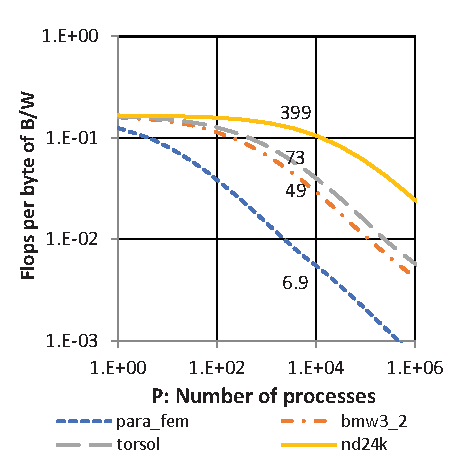
\includegraphics[scale=0.75]{figures/spmv-flop-per-byte-vs-P.eps}
\caption{Scaling in Flops per byte of BW.}
\label{fig:spmv-flop-per-byte-vs-P}
\end{centering}\end{figure}

Dividing this into $2*nnz/P$ (the number of flops per process) yields the number of flops performed per byte of memory bandwidth. Fig. \ref{fig:spmv-flop-per-byte-vs-P} diagrams how this relative performance changes for the same matrices from Fig. \ref{fig:spmv-bylina-speedup} as a function of the number of processes into which the matrix is partitioned. The numbers on each line represent the average number of non-zeros on each row of the full matrix.

%The interpretation of a curve is that for each matrix, if an implementation uses some number of independent processes, then, ignoring the MPI\_reduce and barrier, the performance returned in flops/s should be approximately the number from the curve, times the total memory bandwidth of the system. The key takeaway is that the sparser the matrix, the less effective in terms of delivered flops/s a system will be, with a very rapid decay. 

Assuming that all processes have the same available bandwidth from memory, then multiplying the point on the curve by the number of processes gives the system-wide flops/s per byte/s of memory bandwidth per process. Dividing this into the flops needed for the matrix gives something proportional to execution time. Fig. \ref{fig:spmv-flop-per-byte-vs-P} normalizes this to that for one process, and plots a ``speedup'' number. The ``perfect curve'' on this chart corresponds to a perfect strong scaling reference. It is clear that scaling is sensitive to sparsity, but we don't yet see a dip as in Fig.  \ref{fig:spmv-bylina-speedup}.

\begin{figure}\begin{centering}
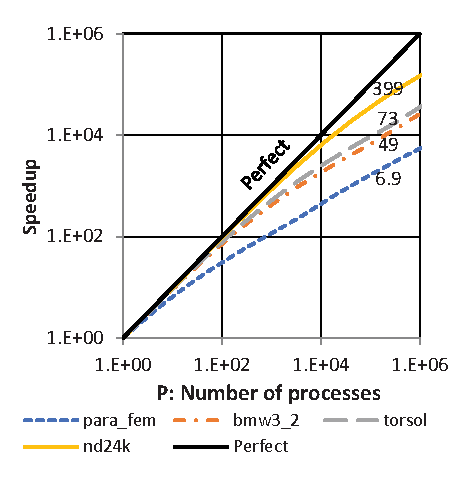
\includegraphics[scale=0.75]{figures/spmv-partial-speedup.eps}
\caption{Single Process Speedup.}
\label{fig:spmv-partial-speedup}
\end{centering}\end{figure}

As a reference, HPCG uses SpMV extensively, but is arranged as a weak scaling problem with a near constant 27 non-zeros per row per process, regardless of the number of processes. Using the above equations, this equates to 0.156 flops per byte of bandwidth, regardless of P. This is in good agreement with the observations from Fig. \ref{fig:spmv-historical-hpcg-bw}.

\subsection{Inter-process Effects}

The above analysis leaves out one important consideration - the effects of required inter-process communication when more than one process is involved in the computation. We ignore here any initial load and distribution of both $A$ and $x$, but not the formation of the final $y$ . Computing the overall $y$ requires accumulating all the segments computed by each process. This is done independently over each row of processes, with each process in a row sending its $N/p$ values via an \emph{MPI\_reduce} into an accumulation vector in the column 0 process in that row. This is then followed by an \emph{MPI\_barrier} to detect completion. Since the length of each segment of $8N/p$ bytes can be quite large (especially for small $p$), many MPI implementations will break the transmission of the full vector into smaller packets, and thus overlap each packet with the reduce computations in the target process.

We consider the \emph{MPI\_reduce} first. A ``PLogP'' pipelined model developed in \cite{techbib:Pjesivac-Grbovic:2007:PAM:1265235.1265248} (that matched experimental data relatively well) estimates the time for such a reduce as:
 
\begin{eqnarray}\label{eq:plogp}
T_{reduce}~=~(P-1)*(L+max(g(m_s),o_r(m_s)+\gamma m_s)) \\
+~(n_s-1)(max(g(m_s),o_s(m_s)+\gamma m_s))~+~o_s(m_s))
\end{eqnarray}

where:
\begin{itemize}
\item $L$ =  the latency of an MPI message between two nodes
\item $m_s$ is the size in bytes of a segment into which MPI divides the input vector
\item $n_s$ is the number of segments into which MPI divides the input vector
\item $o_s(m_s)$ and $o_r(m_s)$ are overheads for send and receive
\item $\gamma$ is the time ``per byte'' to do the reduction at the target
\item $g(m_s)$ is the minimum gap between two messages on the same link
\end{itemize}

A recent presentation \cite{techbib:mvapich2} reported an $MPI\_reduce$ latency on a QDR Inifiniband link (approximating what was in the system we used) as about $140\mu s$ for message segment sizes of 8 bytes and above. Another reference \cite{techbib:Doerfler2006} provides some measurements on the MPI send and receive overheads of about $1-2{\mu}s$. If we want to convert these times into an equivalent memory bandwidth demand, we could multiply by the total memory bandwidth available to a process. For a modern socket with 4 memory channels of 1.866 GB/s each, this converts $1\mu s$ into about $4*1866=7464$ bytes of bandwidth.

$\gamma$ for this reduction should reflect an atomic double float to memory from the incoming data. This is notionally 5 memory accesses of 8 bytes each per 8 bytes of message: a write into the message buffer followed by a read and a write into a user space buffer, a read from that buffer, a read from the target y location, and a final write to the target location.\footnote{It is possible that the latter two are satisfied by cache. With $N/p$ y values this is thus between $8N/p$ and $24N/p$. It is also possible that all three accesses may even be overlapped.} This assumes that no extra memory locations are needed to manage the atomicity of the update. Thus $\gamma$ is the equivalent time to about $5*8/8 = 5$ bytes of memory bandwidth per byte of input. Since it is likely that at least page-sized pieces of the $y$  in a process is in a single memory channel, it is probably appropriate to multiply this by the number of memory channels to convert it into a realistic number.

It is likely that the gap between messages is smaller than the processing term, so $g(m_s)$ can be ignored.

For our problem $n_s=(8N/p)/m_s$, and we approximate $o_s(m_s)=o_r(m_s)=o$. Also, if we define $M$ as the memory bandwidth available to a process in B/s, then we can convert Eqtn. \ref{eq:plogp} from time into an equivalent memory load in bytes of:

\begin{eqnarray}\label{eq:plogp2}
M(P-1)(L+o+\gamma m_s) 
+(8NM/pm_s-1)(2o+\gamma m_s)
\end{eqnarray}

One consideration for the above equation is the $(P-1)$ term which says that each of the $P-1$ processes in the row other than the column 0 process add a separate latency of $L$ to the total. This may not be rational, as its probable that the end-to-end latency from each process is highly overlapped in some way as they all start at roughly the same time. Thus we may want to consider replacing $(P-1)L$ by simply $L$, but leave the $(P-1)$ in front of the other terms, as they are largely serialized on the target process. However, when $P$ is large, this latter term may get excessive, and it may be worth considering an \emph{MPI\_reduce} implementation that performs a log reduction. In this case, assuming a base $Q$ reduction, each level would require a separate $L$, but only $(Q-1)$ repetitions of the latter terms. This leads to the following cases for Eqtn \ref{eq:plogp2}:

\begin{eqnarray}\label{eq:plogp3}
No\_Overlap:~M(P-1)(L+o+\gamma m_s)\\+(8NM/pm_s-1)(2o+\gamma m_s)\\
Overlap:~ML+M(P-1)(o+\gamma m_s)\\+(8NM/pm_s-1)(2o+\gamma m_s) \\
Log_Q:~M*log_Q(P)(L+o+\gamma m_s)\\+log_Q(P)*Q(8NM/pm_s-1)(2o+\gamma m_s)\\
\end{eqnarray}


Finally, the second collective is a barrier at the end between all p processes in column 0. The same ``PLogP'' model from \cite{techbib:Pjesivac-Grbovic:2007:PAM:1265235.1265248} estimates that such time is again a function of $L$, with an extra factor of 2 for the return from the barrier. This would add a term $2ML$ to the above.


%Combining these two terms gives an equivalent bandwidth cost of about $672p-224$ bytes of bandwidth. A backwards curve fit from \cite{techbib:6933066} estimated an equivalent term at about 3600 for a $4x4$ process array, indicating that we are in the right ballpark.

\subsection{A Common Model}

\begin{figure*}\begin{centering}
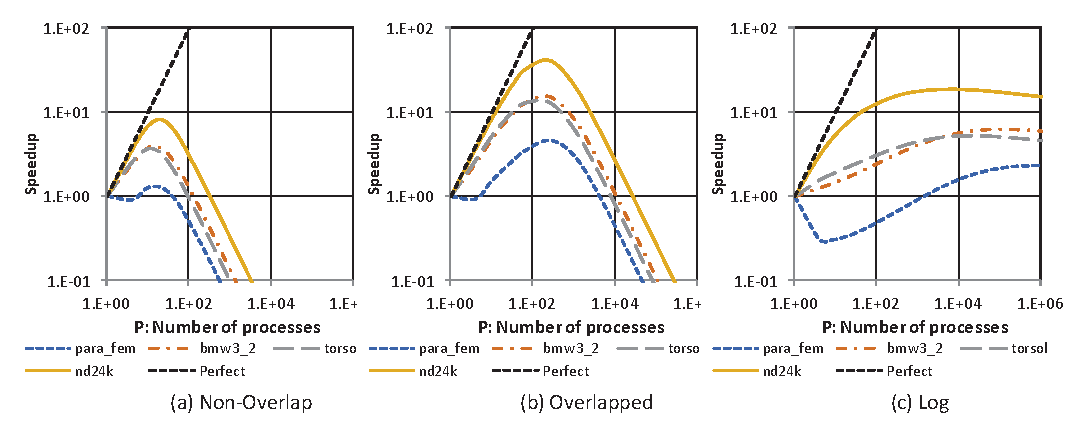
\includegraphics[scale=0.85]{figures/spmv-analytic-model.eps}
\caption{The Three Models.}
\label{fig:spmv-analytic-model}
\end{centering}\end{figure*}

For an estimate of the memory load on a process in column zero in terms of memory load, we can add Eqtns. \ref{eq:1process} and one of \ref{eq:plogp3}, along with a term $2ML$. Fig. \ref{fig:spmv-analytic-model} diagrams these three models as speedup numbers, where the time for the reference single process is in fact that for just the local computations, with no reduce or barrier.

For the Non-Overlapped and Overlapped cases, the speedups for the denser cases are fairly good up to a certain point (about $6x6$ for the Non-Overlapped and $10x10$ for the Overlapped), after which speedups actually decline. This is due to the sparsity per local row in each process dropping below a critical point where overhead now dominates, as the number of processes that have to be serially summed together into the column 0 becomes large. The sparsest case is even worse, and in fact gains very little until a moderate amount of parallelism is present.

The Log case is most inserting in that it matches the shapes of Fig. \ref{fig:spmv-bylina-speedup} very well, at least up to the limited process array sizes in Fig. \ref{fig:spmv-bylina-speedup}.  Thus we suspect that the MPI implementation used in \cite{techbib:6933066} was probably an ``optimizing'' version that performed a logarithmic approach to multiple reductions. In particular, this set of curves includes the pronounce dip in performance for the sparsest case at small numbers of concurrency. Further, this case does not experience the actual declines in speedup at larger systems, but essentially goes flat.

